% Proton is made out of partons (quarsk + gluons) which contain a colour charge resulting in an interaction called the strong interaction. The theory describing this interaction is called QCD.

% Coupling constant depends on the energy scale of the interaction. 

%\begin{frame}{Outline}
%
%\vspace*{\titleskip}
%
%	\begin{enumerate}
%		\item {\textbf{Motivation}}
%		\begin{itemize}
%			\item What are parton distribution functions (PDFs)?
%			\item Why do we want to determine them?
%		\end{itemize}
%		
%		\item {\textbf{Methodology}}
%		\begin{itemize}
%			\item The Machine Learning problem
%			\item The NNPDF methodology
%		\end{itemize}
%
%		\item {\textbf{Removing bias}}
%		\begin{itemize}
%			\item Simplified architecture
%			\item The extrapolation region
%		\end{itemize}
%		
%		\item{\textbf{Outlook}}
%		
%	\end{enumerate}
%	
%\end{frame}


\section{Motivation}

%\begin{frame}{Quantum Chromodynamics}
%
%\vspace*{\titleskip}
%
%\begin{columns}[T,onlytextwidth]
%	\column{0.70\textwidth}
%	\begin{itemize}
%
%		\item The theory of the \textbf{strong interaction} is called \textbf{Quantum Chromodynamics (QCD)}
%
%
%		\item Hadrons are made up out of \textbf{partons} bound by gluons
%		
%		\item Quarks carry fractional electric charge
%
%		\item Quarks posses a property called \textbf{colour  charge}
%		
%	\end{itemize}
%	\column{0.05\textwidth}
%	\column{0.25\textwidth}
%	\vspace*{0pt}
%	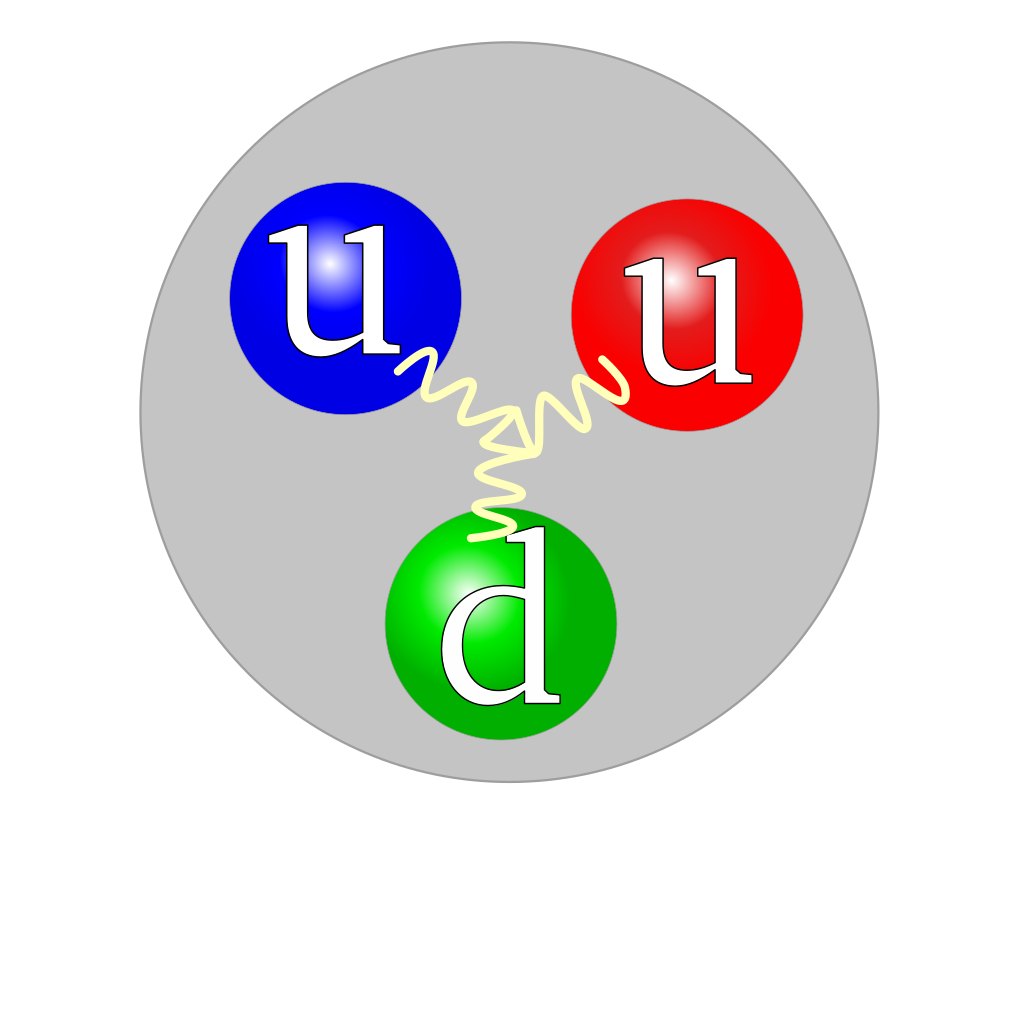
\includegraphics[width=0.95\textwidth]{proton_structure_uud}
%\end{columns}
%
%
%\end{frame}
%
%%=============================================================
%
%\begin{frame}{Quantum Chromodynamics}
%
%\vspace*{\titleskip}
%
%\begin{itemize}
%	\item The strength of the interaction is described by the strong coupling constant $\alpha_s$
%	
%	\item $\alpha_s$ decreases as the  energy increases
%	
%	\item In the high energy limit, perturbative cross section can be calculated
%	
%\end{itemize}
%
%\end{frame}

%=============================================================


%\begin{frame}{Parton distribution functions (PDFs)}
%
%\vspace*{\titleskip}
%
%\begin{columns}[T,onlytextwidth]
%	\column{0.70\textwidth}
%	\begin{itemize}
%	
%	\item PDFs describe the partonic substructure of hadrons
%
%	\item PDFs are needed to provide a theoretical prediction for particle physics experiments
%	
%	\end{itemize}
%	\column{0.05\textwidth}
%	\column{0.25\textwidth}
%	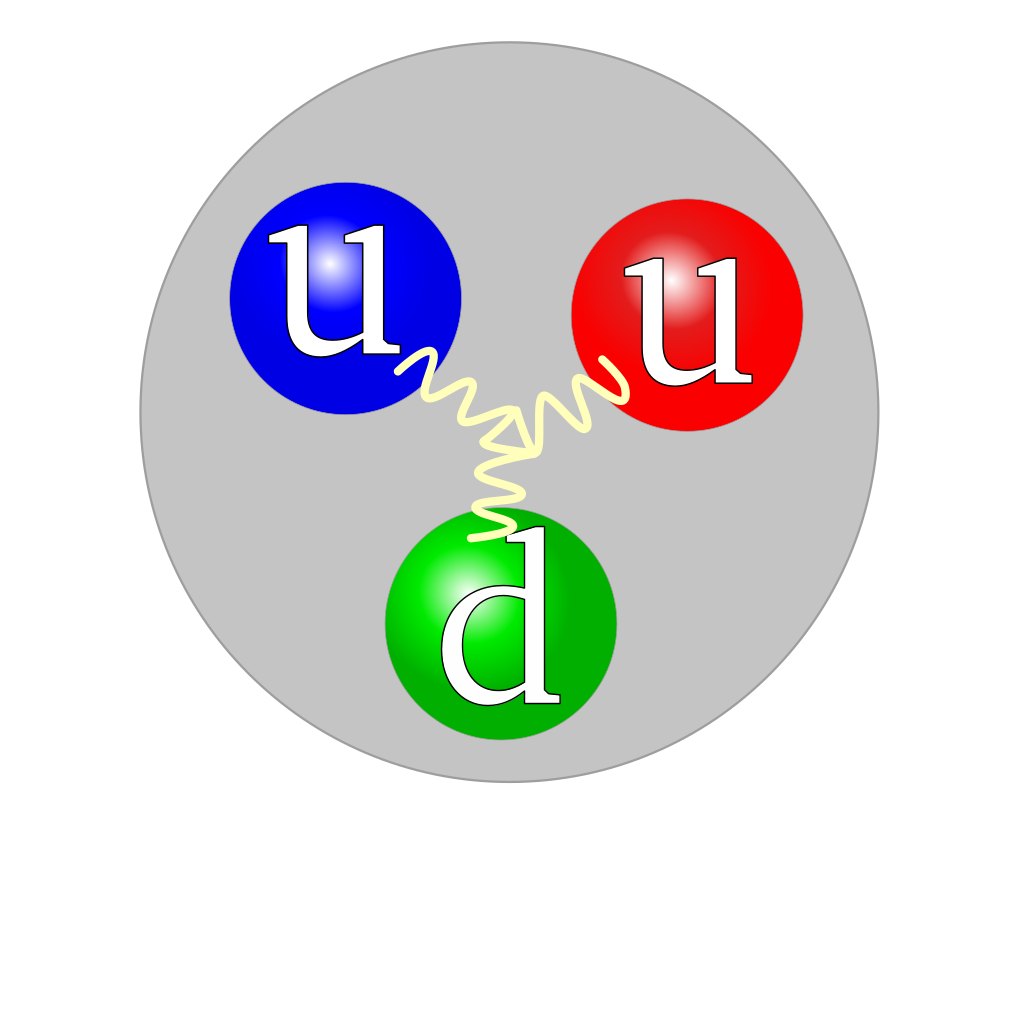
\includegraphics[width=0.95\textwidth]{proton_structure_uud}
%\end{columns}
%
%
%\end{frame}

\begin{frame}{Parton distribution functions (PDFs)}

\vspace*{\titleskip}

\begin{itemize}
	\item PDFs are required to provide theoretical predictions	

	\item Hadron collisions are factored into a 'hard part' $\hat{\sigma}$ and a normalization provided by the PDFs	
	
	\item We cannot calculate PDFs
	
%	\item PDFs are a universal property of a hadron
	
%	\item We do not have reasons to assume a functional form of the PDFs	
	
\end{itemize}

\begin{center}

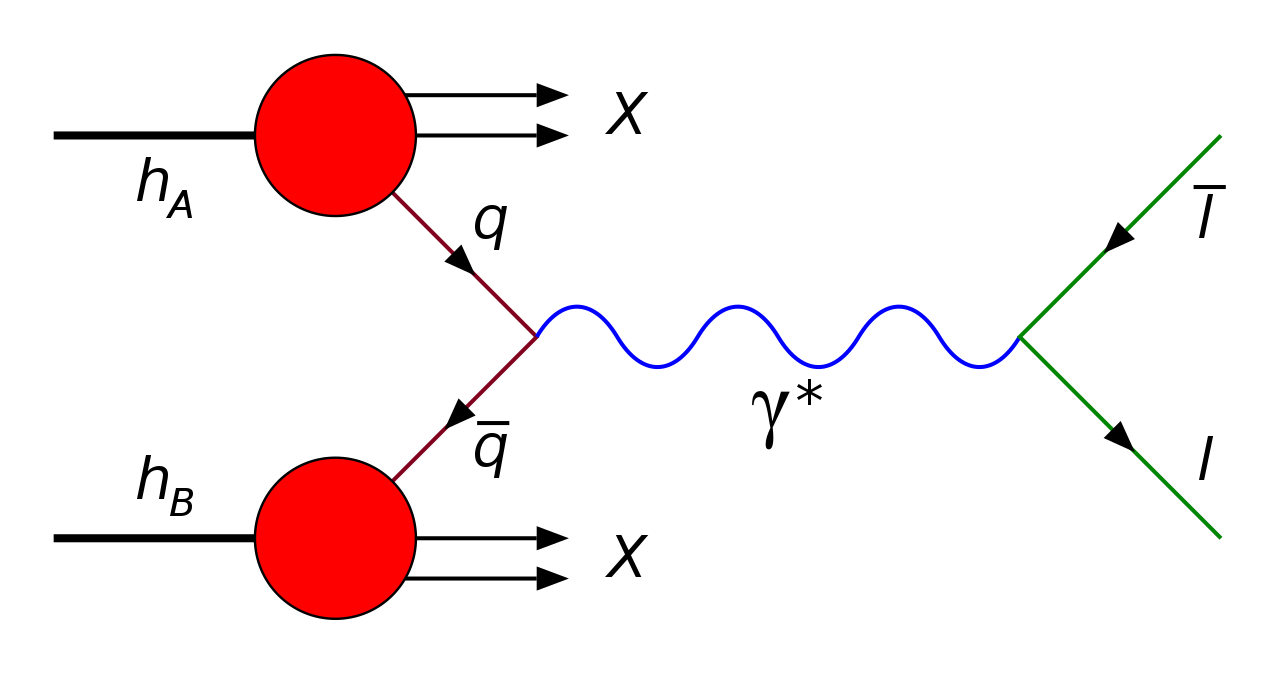
\includegraphics[width=0.5\textwidth]{Drell-Yan}

\vspace{-0.5cm}
$$ \overbrace{\sigma_X}^{\text{experiment}}=\sum_{a, b} \int d x_{1} d x_{2} \overbrace{ f_{a / h_{A}}\left(x_{1}\right) f_{b / h_{B}}\left(x_{2}\right)}^{\text{PDFs}} \overbrace{ \hat{\sigma}_{a b \rightarrow X}}^{\text{theory}} $$
%$$ \overbrace{\sigma_X\left(s,\mu^2\right)}^{\text{experiment}}=\sum_{a, b} \int_{0}^{1} d x_{1} d x_{2} \overbrace{ f_{a / h_{A}}\left(x_{1}, \mu^{2}\right) f_{b / h_{B}}\left(x_{2}, \mu^{2}\right)}^{\text{PDFs}} \overbrace{ \hat{\sigma}_{a b \rightarrow X}\left(\mu^{2}\right)}^{\text{theory}} $$

\end{center}


\end{frame}

%=============================================================

%\begin{frame}{Parton distribution functions}
%
%\vspace*{\titleskip}
%An accurate determination of PDFs is needed to determine the expected observables for an experiment.  
%\vspace*{\secondskip}
%
%\begin{center}
%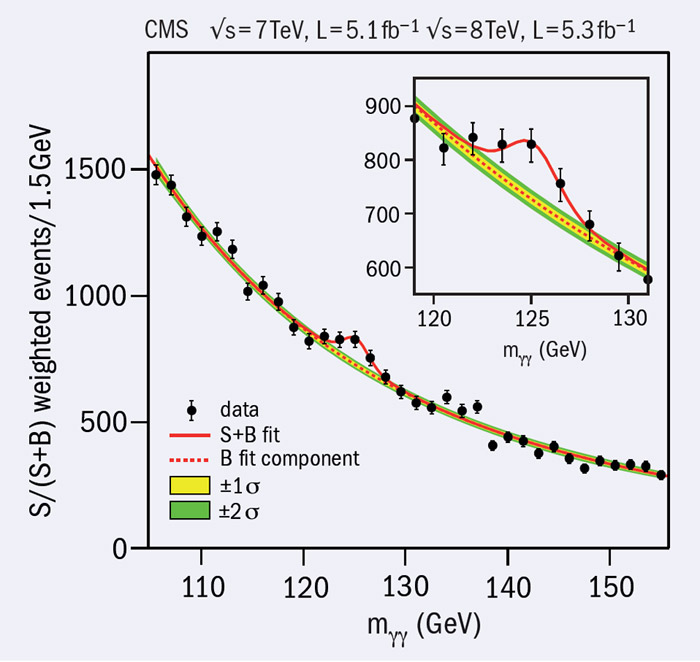
\includegraphics[width=0.5\textwidth]{Higgs_measurement}
%\end{center}
%
%\end{frame}

%=============================================================

\section{Methodology}

\begin{frame}{The NNPDF collaboration}

\vspace*{\titleskip}

%
\includegraphics[width=1.0\textwidth]{NNPDF_N3PDF_arrow}
\begin{center}

\includegraphics[width=0.4\textwidth]{nnpdflogo_noback}
\end{center}

\vspace*{\secondskip}

\begin{itemize}
	\item NNPDF provides PDF determination using Neural Networks
%	\item Aim: Unbiased results 
\end{itemize}

\end{frame}

%=============================================================

%\begin{frame}{The fitting problem}
%
%\vspace*{\titleskip}
%
%\begin{itemize}
%	
%\item First fitting attempt: $f_i=A_ix^{\alpha_i}(1-x)^{\beta_i}$
%	
%\item Based on arguments in the limits $x\rightarrow 0$ and $x \rightarrow 1$
%
%%\item PDFs are scale dependent 
%
%\item Assuming a functional form leads to underestimation of PDF uncertainties
%
%%\item This can be overcome by using a neural network
%	
%\end{itemize}
%
%\vspace*{\secondskip}
%
%\begin{center}
%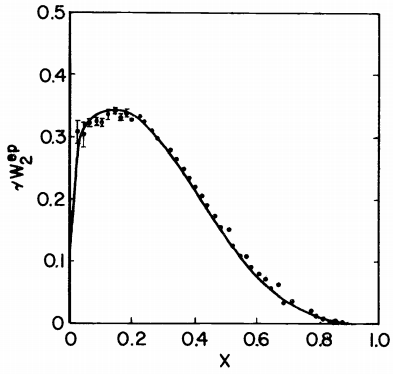
\includegraphics[width=0.3\textwidth]{first_pdf}
%\end{center}
%
%\end{frame}

%=============================================================

\begin{frame}{The NNPDF methodology}

\vspace*{\titleskip}

\begin{itemize}
\item Using a Neural Network reduces bias from the functional form
\begin{itemize}
\item $f_i=\text{A}_ix^{\alpha_i}(1-x)^{\beta_i}\text{NN}_i(x,\log x)$
\end{itemize}
\item Monte Carlo set of PDFs
\item Minimization using gradient descent 
\item Stopping based on training/validation data
\end{itemize}

\vspace*{\secondskip}

\begin{columns}[T,onlytextwidth]
	\column{0.475\textwidth}
	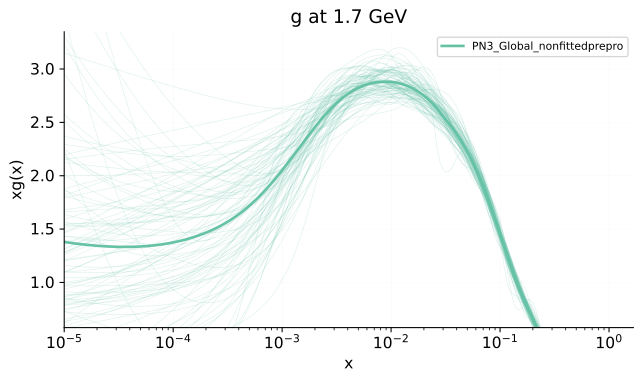
\includegraphics[width=\textwidth]{pdfreplicas}
	\column{0.05\textwidth}
	\column{0.475\textwidth}
	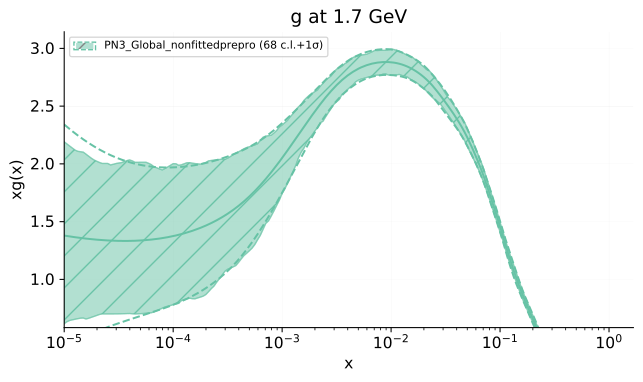
\includegraphics[width=\textwidth]{pdfplot}
\end{columns}

\end{frame}

%=============================================================

\section{Removing bias}


\begin{frame}{Bias}

\vspace*{\titleskip}
The methodology is still not completely free of bias $f_i=\text{A}_ix^{\alpha_i}(1-x)^{\beta_i}\text{NN}_i(x,\log x)$

If preprocessing is removed, we observe saturation at small-x:
\vspace*{\secondskip}

\begin{center}
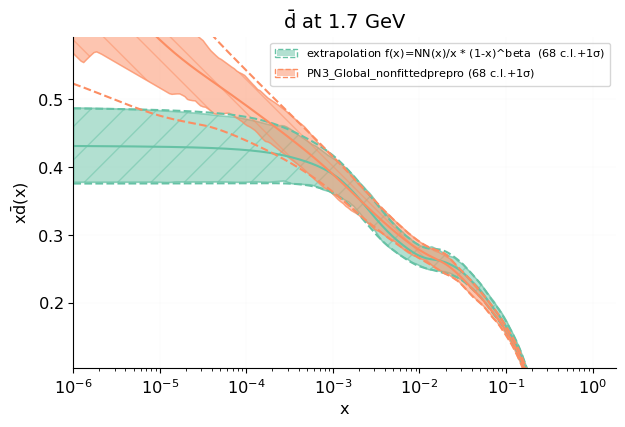
\includegraphics[height=0.3\textwidth]{flatdbar}
\end{center}

\end{frame}

%=============================================================

\begin{frame}{Feature Scaling}

\vspace*{\titleskip}

Solution:
\begin{enumerate}
\item<1-|alert@1-3> Scale the input xgrid such that it is homogeneously distributed
\item<1-|alert@4> Select one in $n$ points  
\item<1-|alert@5> Provide a monotonically increasing interpolation
\end{enumerate}

\only<1-5>{{ Result: $f_i=\text{A}_i \left(\text{NN}_i(x')-\text{NN}_i(1)\right)$}}
\only<6>{\alert{ Result: $f_i=\text{A}_i \left(\text{NN}_i(x')-\text{NN}_i(1)\right)$}}

% figures of xgrid histogram, or maybe simple example of 1D grid of points
\begin{center}
\only<1>{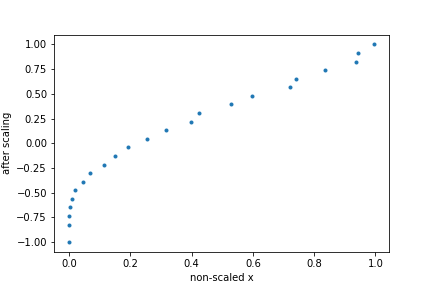
\includegraphics[height=0.3\textwidth]{feature_scaling_1}}
\only<2>{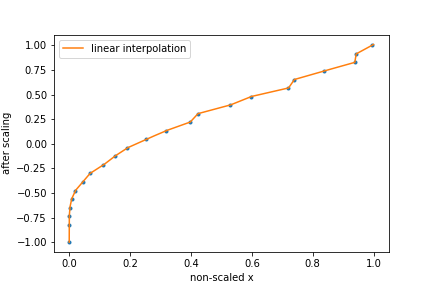
\includegraphics[height=0.3\textwidth]{feature_scaling_2}}
\only<3>{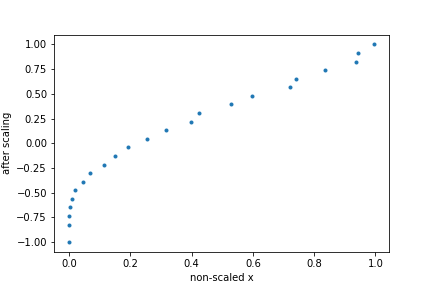
\includegraphics[height=0.3\textwidth]{feature_scaling_1}}\only<4>{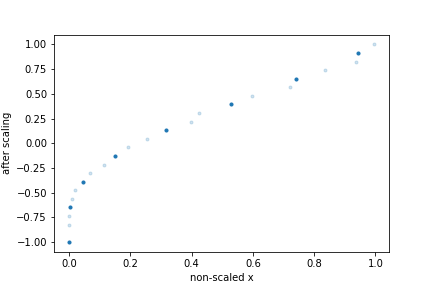
\includegraphics[height=0.3\textwidth]{feature_scaling_3}}\only<5>{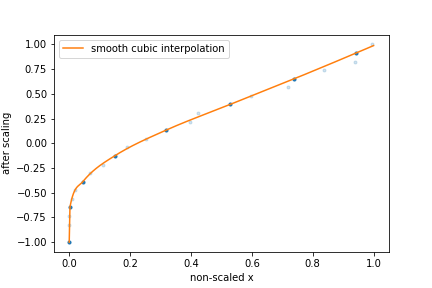
\includegraphics[height=0.3\textwidth]{feature_scaling_4}}
\only<6>{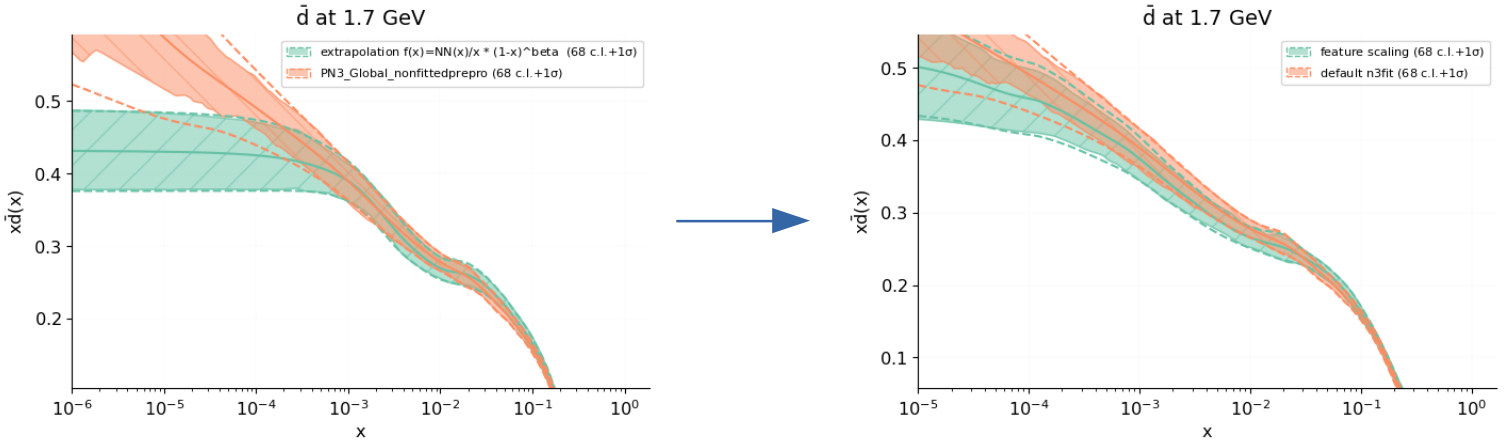
\includegraphics[height=0.3\textwidth]{flat_to_feature}
}
\end{center}

\end{frame}


%=============================================================

\begin{frame}{Outlook: the extrapolation region}

\vspace*{\titleskip}

\begin{itemize}
\item Now we no longer have any prediction for the extrapolation region
\item Use Gaussian Process Regression to fit observables + uncertainty
\item Generate observables in the extrapolation region
\item Include this Gaussian pseudodata in the NNPDF fit
\end{itemize}

\vspace*{\secondskip}

%\begin{columns}[T,onlytextwidth]
%	\column{0.475\textwidth}
%	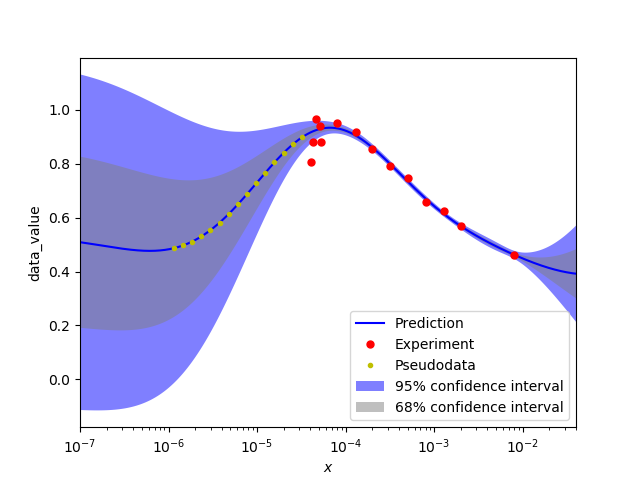
\includegraphics[width=\textwidth]{GP}							\column{0.05\textwidth}
%	\column{0.475\textwidth}
%	\vspace{0.7cm}
%	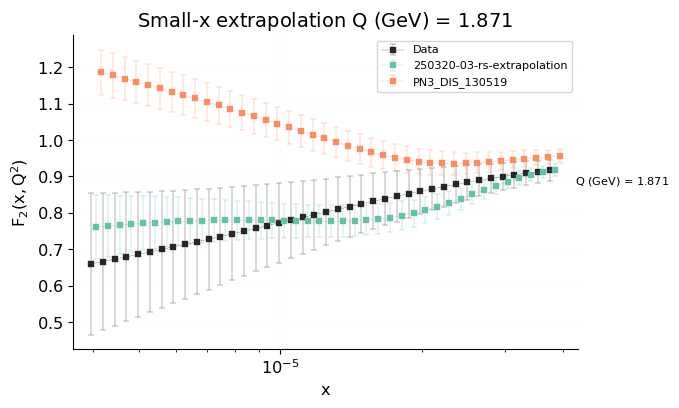
\includegraphics[width=\textwidth]{preproc_dominates_smallx}
%\end{columns}

\begin{center}
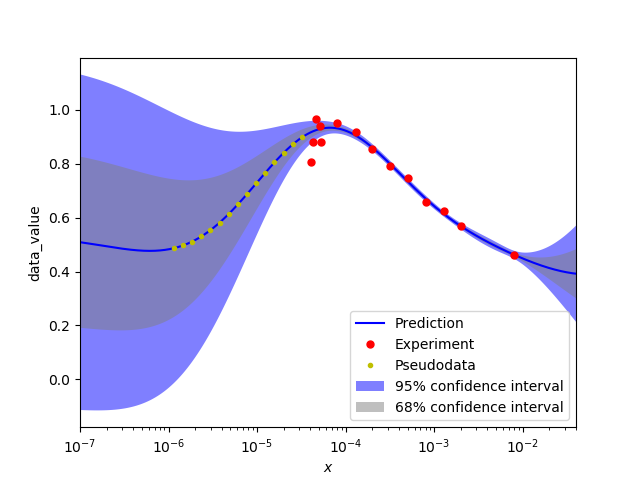
\includegraphics[width=0.5\textwidth]{GP}
\end{center}


\end{frame}

%=============================================================


%\section{Conclusions}
%
%
%\begin{frame}{Conclusions and Outlook}
%
%\vspace*{\titleskip}
%
%Conclusions:
%	\begin{itemize}
%		\item PDFs are needed to make the connection between theory and experiment
%		
%		\item Machine Learning reduces bias in PDF determination
%		
%		\item We have shown a method to reduce bias even further
%		
%		\item Outlook: provide a prediction in the extrapolation region
%				
%	\end{itemize}
%
%\end{frame}

%=============================================================

{
\setbeamercolor{background canvas}{bg=mDarkTeal}
\begin{frame}[plain,noframenumbering]
\vspace{0.5\textheight}
\centering \Large \color{white} \textbf{Thank you!}
\end{frame}
}